\chapter*{Introduction}
\markboth{Introduction}{Introduction}
\addcontentsline{toc}{chapter}{Introduction}


\begin{quote}{K. Yamaguchi}
	“Clothing recognition is a challenging and societally important problem – global sales for clothing total over a hundred billion dollars, much of which is conducted online." \cite{yamaguchi2013paper}
\end{quote}

You can already see the impact Deep Learning has been giving to many sectors in recent years, and clothing recognition has been one of the last ones to reach an acceptable level of confidence in the results.

Here's an example of a successful apparel recognition:

\begin{figure}[H]
	\centering
	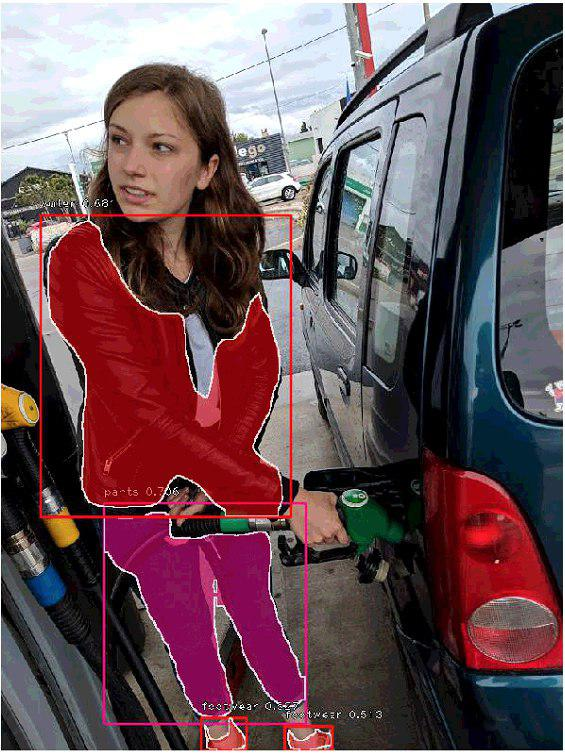
\includegraphics[width=.5\linewidth]{images/difficultscenario.jpg}
	\caption{Successful recognition in a real-world image. Sorry for the unfortunate image of a French petrol station, we definitely should have taken the image in an EV charging station!}
\end{figure}

As you can see, it recognized footwear, pants, and the macrocategory “outer" that includes jackets etc. The table with all the labels is available in \sref{s:ds-modanet}.

The program also drew the edges around each object, along with drawing a colored box matches the label. This allows for segmenting the image into all the objects that are in the scene (and that we are interested in recognizing).
More details on \emph{Instance Segmentation} available in \sref{s:ltask-patt}, and more specifically in \sref{s:patt-insta}.

So, we've learned what the task is. How does the algotithm learn, though?

It learns by example. In my particular case, it is given 50 thousand images, along with annotations for each image -- which tell the algorithm what are the patterns to detect that characterize each object, and are formatted just as the results: bounding boxes, labels and masks (that's how the object's edge and inside is called). More details on the dataset in \modanet.

The algorithm we are talking about and that I was advised to use by the researchers at IMP Lab (where I wrote this), is called \maskrcnn. It is the last in a series of developements (it was only developed less than two years ago), described in detail in \sref{s:nnevo}.

Onto the next question you probably have, if you're still reading!
What could the applications of such an algorithm be?

Well, this thesis is marketed to us students as being commissioned by Adidas, so it's evident that there's at least \emph{some} interest in this by apparel companies.
The reasoning is: it's easy for us humans to detect things around us and be able to describe them accurately; our mind works similarly to a neural network [basics described in \sref{s:perc}].
Just like robots conquered our factories, digital ones are conquering social networks:
for example there's recently been a notable effort to reduce fake news and nudities on these platforms. One can simply not expect a human to be able to scan through millions of images (or billions!). 

In fact:
\begin{quote}[theatlantic.com]{Rose Eveleth}
	“In 2014, according to Mary Meeker's annual Internet Trends report, people uploaded an average of 1.8 billion digital images every single day. That's 657 billion photos per year."
\end{quote}

This leads us to the opportunites of an algorithm with these capabilities.
From analyzing how an apparel item is used, where, and with whom -- friends, coworkers, your significant other -- furthermore to measure how well of an impact, \emph{Creators} (called “Influencers" in Italy) are making in a rapidly evolving environment in which marketing is more and more based on trust between people you know and follow, rather than from stars from Hollywood that are becoming less and less important as a model to follow.
And this radical shift requires new data analytics tools just as ours and the developements it will have in the future.


